PREESM is a rapid prototyping framework for multi-core development. For understanding the OpenEM framework a way to construct comparable programs with different multi-core runtime was needed. PREESM provides a way to quickly construct multi-core applications for PC as well as for the Texas Instruments multi-core DSP used in the experiments. In this chapter the PREESM framework is introduced. First, an overview of the framework is given in subsection \ref{subsec:preesm-overview}. Second, the framework overview, the internal representations used by the framework are described in subsection \ref{subsec:preesm-internal}. Third, scheduling in the PREESM framework is explained in subsection \ref{subsec:preesm-scheduling}. And Finally, the code generation in PREESM is explained in subsection~\ref{subsec:preesm-codegen}.

\subsection{PREESM Overview}
\label{subsec:preesm-overview}
PREESM is a collection of tools for rapid prototyping multi-core applications. The tools include a graphical editor for the hardware and the software models, code generators for multiple hardware platforms and an automated generator for fixed schedules. The PREESM tools are used through the Eclipse IDE based environment available at~\cite{preesm}.

In PREESM prototypes of applications are constructed by combining hardware and software models with manually created source code and automatically generated schedule. The software model used in PREESM is based on dataflow models of computation and it is discussed in detail in subsection \ref{subsubsec:preesm-algorithm}. To create a software model in PREESM the application is divided into actors. The actors contain manually created code, which is often written in side-effect free style to enable parallel execution of the actors, but this is not enforced by the framework. The graphical editor for the software model allows the user to create actors and connect them together using first in first out queues.~\cite{preesm}

The model of the target hardware platform is created using a similar graphical tool as the software model. The hardware model is described in subsection \ref{subsubsec:preesm-hardware}. PREESM parses the graphs of the models and creates a static schedule for the executable. The schedule, the actor implementations and the graphs are inputs for the code generator, which creates the multi-core executable.~\cite{pelcat2014preesm} The graphical tools allow the PREESM user to create dependencies between the actors. They also allow a more fine grained control over the code generation by setting estimated actor execution times and selecting the cores on which each actor is allowed to execute.

\begin{figure}[h!]
    \begin{center}
        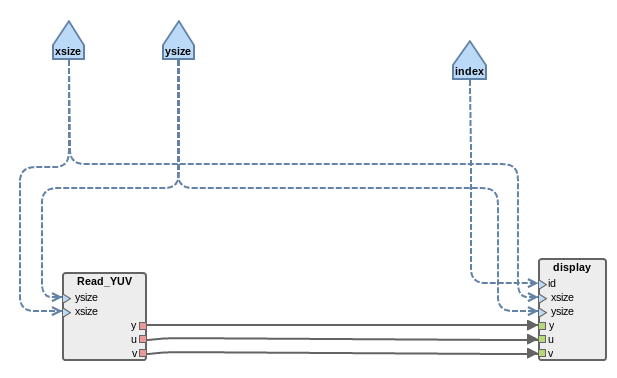
\includegraphics[width=0.99\textwidth]{images/example_preesm_diagram.png}
        \caption{A simple dataflow diagram created with PREESM.}
        \label{fig:preesm_example}
    \end{center}
\end{figure}

\subsection{PREESM Internal Representations}
\label{sec:dataflow}
PREESM applications are created by combining inputs of two different internal representations and manually created source code. The two internal representations are described here: first the PREESM algorithm representation PiSDF and second the PREESM hardware model.

\subsubsection{PREESM Algorithm Representation}
The PREESM applications are defined using the Parameterized and Interfaced Synchronous Dataflow Model of Computation (PiSDF)\cite{pelcat2014preesm}. \fixme{detached}

Dataflow Model of Computation (MoC) is a directed graph where each node represents a function and the arcs are the only possible paths the data can traverse in the graph. In the generic Dataflow MoC the number of tokens produced or consumed by an actor is not known before execution. For example an actor may have two output paths and it may choose to produce an output token conditionally to either one (or both) of the paths. In contrast in Synchronous Data Flow (SDF) MoC each actor produces and consumes a pre-determined number of tokens. \cite{lee1987synchronous} A more thorough explanation of Dataflow MoCs can be found in \cite{lee2015introduction}.

PREESM uses an extended version of SDF called PiSDF \cite{pelcat2014preesm}. PiSDF extends SDF by providing hierarchical graphs based on interfaces and by introducing parameterized actors. An actor in PiSDF can be replaced by a subgraph, which has input and output interfaces. The interfaces insulate the hierarchy levels in terms of schedulability analysis. The parameters are used to reconfigure the production and consumption rates of the actors. \cite{desnos2013pimm} An example of a PiSDF graph is presented in figure \ref{fig:preesm_example}. The parameters of the PiSDF model are presented at the top of the figure as pentagons connected to the actors with dashed lines. The actors have input and output ports for parameters and data. The ports define the input and output interfaces of the actors. The actual data paths are the arcs connecting the actors in the bottom of the figure.

\subsubsection{PREESM Platform Representation}
The PREESM code generation is aware of the target hardware platform. PREESM uses System-Level Architecture Model (S-LAM) \cite{pelcat2009system} to describe the target architecture. S-LAM is designed specifically to provide architecture models of high asbtraction level for rapid prototyping purposes. S-LAM is suitable for modeling heterogeneous architectures as a S-LAM can contain different types of computational resources and communication links. PREESM calculates the speeds of the connections in the S-LAM and takes them into account when creating a static schedule. \cite{pelcat2009system}

PREESM provides graphical tools for editing the S-LAM. For example the S-LAM representing the TMS320C6678 used in experiment \ref{sec:firstexperiment} is quite simple consisting of eight c6678 cores connected through shared memory.

\subsection{PREESM Scheduling}
\label{sec:preesmsched}
A general problem in the design of multicore applications is efficient scheduling. The PREESM framework generates a schedule for multicore platforms using the \textit{List} and \textit{Fast} scheduling methods explained in \cite{kwok1997high}. The PREESM framework focuses on latency dominated systems where respecting the latency constraints guarantees fulfilment of the throughput constraint \cite{pelcat2014preesm, ghamarian2006throughput}. Because the scheduler only considers the latency of the execution, the iterations of the algorithm are not interleaved. Instead, all cores are synchronized between the iterations with a barrier. Intra-iteration interleaving is supported by the PREESM scheduler. \cite{pelcat2014preesm} An example of the intra-iteration interleaving is given in the software pipelining tutorial available at \cite{preesm} \fixme{what does intra-iteration interleaving actually mean}. The estimated execution times for each actor are provided by the user. PREESM framework visualizes the generated schedule with a gantt chart. An example gantt chart is presented in figure \ref{fig:preesm_gantt}.\\ \fixme{This doesn't need to be so condensed, make it more verbose.\\ explain wtf is going on with the explode and implode stuff \\ how does the preesm inter actor communication work in detail \\ explain preesm memory usage}
